%`
%Read /home/ocean/Documents/PTNR/CulhamFusion/AllPapers/ANNunfolding/BonnerSphere/ThreeAIUnfolding.pdf
%\nonstopmode
\hbadness=100000
\documentclass[a4paper, 12pt]{article}
\usepackage{amsmath,amsfonts,changepage,caption,float,geometry,graphicx,mathtools,pythonhighlight,textcomp,url,verbatim,subcaption} %,parskip
% \usepackage[justification=centering]{subfig}
\geometry{ a4paper, total={170mm,257mm}, left=20mm, top=20mm}

\newcommand{\matr}[1]{\underline{\underline{\textbf{#1}}}}
\newcommand{\ve}[1]{\boldsymbol{#1}}
\newcommand{\pythoncode}[2]{
\begin{adjustwidth}{-1.3cm}{-1.3cm}
\texttt{#1}
\inputpython{#2}{1}{1500}
\end{adjustwidth}
}
\newcommand{\fluenceandactivities}[1]{
\includegraphics[width=11cm]{#1fluence.png}
\includegraphics[width=5cm]{#1activities.png}
}
\usepackage[toc, page]{appendix}
% \usepackage[dvipsnames]{xcolor}
% \definecolor{subr}{rgb}{0.8, 0.33, 0.0}
% \definecolor{func}{rgb}{0.76, 0.6, 0.42}

\begin{document}

\centering


\includegraphics[width=8cm]{CoverPage/UoBlogo.pdf}
\hrule
\bigbreak
\textbf{F}usion Neutron \textbf{Acti}vation Spectra \textbf{U}nfolding by \textbf{N}eural \textbf{N}etworks \\
(FACTIUNN)                                      \\
\hrule
\bigbreak
\begin{minipage}[b]{0.4\textwidth}
    
\includegraphics[height=2cm]{CoverPage/CCFElogo.jpeg}
  \end{minipage}
  \hfill
  \begin{minipage}[b]{0.4\textwidth}
    
\includegraphics[height=3cm]{CoverPage/UKAEAlogo.jpeg}
\end{minipage}
    
\begin{table}[!h]
\centering
\begin{tabular}{rl}
author:&Ocean Wong          \\
       &(Hoi Yeung Wong)    \\
supervisor:&Ross Worrall    \\
Submitted in fulfilment of the requirement for:& MSc. Physics and Technology of Nuclear Reactors \\
date:  &June-September 2019 \\
student ID:& 1625143        \\
\end{tabular}
\end{table}
\hrule
\bigbreak
I warrant that the content of this dissertation is the direct result of my own work and that any use made in it of published or unpublished materials is fully and correctly referenced.

\abstract
Include these things:
\begin{itemize}
    \item Attempted this
    \item Got this result
    \item advice for the future
\end{itemize}
\emph{Keywords:} activation, neutronics, fusion
% \hline
% \twocolumn
\pagebreak
\tableofcontents
\listoffigures
\pagebreak


\chapter{}
\section{Introduction}
%multicols %for two columns % switch by column break.
% \begin{align}
% 	q=\left[\cos(\frac{\theta}{2}),
% 			x\sin(\frac{\theta}{2}),
% 			y\sin(\frac{\theta}{2}),
% 			z\sin(\frac{\theta}{2})
% 			\right]\\
% \intertext{where}
% \begin{pmatrix}
% 	cov(m,m) & cov(m,c)\\
% 	cov(c,m) & cov(c,c)
% \end{pmatrix}
% \end{align}
    
%Bullshit something about the importance of Fusion later in this paper.

In a fusion reactor, the neutron fluence can go up to as high as $1.6 \times 10^{21}$[citation needed]. (For JET, [citation needed]; for ITER, [citation needed]). This leads to an unprecedented need of shielding against neutrons of up to 14.1 MeV or higher energies, which has not been experienced in fission reactors before [citation needed].

Neutrons are notoriously difficult to shield against due to their uncharged nature, and therefore low propensity to interact with matter[citation needed]. To develop effective shielding for various components of the reactor from these high energy neutrons, the energy spectrum of the neutrons created inside the nuclear reactor has to be well understood[citation needed]. It is also important to understand the neutron spectrum inside the reactor in order to develop Tritium breeding modules, which is essential for making fusion a sustainable source of clean energy. [citation needed]
%Can expand on the Tritium breeding part.
An accurate measurement of the neutron spectrum is required to properly model the energy distribution of neutrons to be used in neutron transport simulations for the above purposes.
% Additionally, knowing the energy distribution of neutrons is beneficial to advancing the current understanding of the the nuclear processes and scattering interactions inside the reactor [citation needed].

Therefore, neutron energy measurement is a key focus [rewording needed] in the diagnostic systems in all fusion reactors.

Ironically, for the same reason that they are difficult to shield against, neutron energy is also difficult to measure. Neutrons, especially high energy neutrons such as the 14.1 MeV neutrons created in fusion reactors, do not easily deposit their full energy into a sufficiently small detection volume to allow direct measurement[citation needed]. Various neutron detectors has been developed to deal with this problem;
[citation needed] %Cite any neutron detector, e.g. organic
%Including magnetic proton recoil?
%And fission chambers (energy indep), neutron cameras
however, most of them cannot stand this high neutron fluence that is found at the first wall of fusion reactors without additional shielding that changes the flux profile, defeating the objective of trying to measure neutrons energy distribution with minimal disturbance to the spectrum itself.[citation needed]
The extreme temperature and magnetic fields inside the nuclear fusion reactor compounds the difficulty of employing other means of neutron measurement as most electronics will not be able to function in such environments effectively.
%List the other two, but say that neutron activation stands out in the following way:

This is where the technique of neutron activation stands out: 

By analyzing the level of activations in various elements induced by neutrons, relying on the fact that different reactions has different sizes of reaction cross-sections, each with varying sensitivities to neutrons of different energies, one can infer the neutron spectra that was previously present at the first wall.

This is a very robust method as it does not require any active components, thus can be employed for very high neutron fluxes and fluences [citation needed], as the total number of neutron activation reactions can be controlled by changing the thickness of the activation foils used [citation needed] according to the anticipated neutron fluence in the next campaign, so not to paralyze the $\gamma$ radiation detector.

The disadvantage of this method is that it has to be time-integrated (over the whole campaign), i.e. no information about the temporal variation in neutron flux can be extracted. [citation needed]

Another disadvantage of using neutron activation as the means of measuring the neutron spectrum in a fusion reactor is that it is an indirect method of measurement, requiring the measured reaction rates to be `unfolded' back into reaction rates. This is a `mathematically incorrectly posed ' problem\cite{BirminghamUnfolding}, as will be further explained in the next section (\ref{Neural Network Theory}), requiring an \emph{a priori} spectrum to be provided before the unfolding procedure can take place. This is because the number of activities recorded (usually denoted as M) is fewer than the number of neutron groups (usually denoted as N) of whose activity we would like to know, i.e. M$<$N, thus the problem is underdetermined (the number of contraints is fewer than the number of variables). The \emph{a priori} has to be used in order to introduce extra information into the problem. However, if this \emph{a priori} spectrum deviates too much from the actual spectrum, then the result of the unfolding will be inaccurate.

To address this problem, an investigation into using neural networks for the purpose of unfolding is presented in this thesis.
Neural networks excels in incorperating previous spectra as \emph{a priori} information, without requiring users to explicitly input an \emph{a priori}.
Two approaches are proposed. The first one is to use neural networks directly as an unfolding tool; and the second one is to use them as an \emph{a priori} generator, which is then fed into an existing unfolding code, where the actual neutrons spectra is then calculated out of.

\section{Theory}
When a nuclide is placed in the activation module at the irradiation position inside a nuclear fusion reactor (or any other neutron sources), it is activated via one or more nuclear reactions with the incoming neutrons. The probability of interacting with the incoming neutron via reaction $j$ is proportional to the microscopic cross-section $\sigma_j (E)$, where $E$ is the neutron's energy, and reaction $j$ is a neutron-induced reaction, i.e. (n,??) reaction.

% The measured activity = (count rate)/(absolute efficiency of set-up at energy for decay of daughter j) /(count period);
% The total number of reaction $j$ = (measured activity)/(probability of daughter's gamma decay per second)

By measuring the activity of reaction $j$'s daughter nuclide in the activation foil (which has a known amount of the initial nuclide) after irradiation, and multiplying it by a correction factor of 
\begin{equation}
    \frac{1}{{1-exp({\lambda_j}T)}}
\end{equation}
the reaction rate $Z_{0j}$ can be obtained. This correction factor accounts for the decay of the daughter nuclide of reaction $j$ which has a half-life of $\lambda_j$, over the period $T$ which is the duration between irradiation and measurement. A more complicated correction factor is required if the irradiation period is comparable to the half-life $\lambda_j$, or if the population of the parent nuclides for reaction $j$ changes over the course of the irradiation. This can be done using FISPACT-II, detailed in [citation needed].

The total reaction rate of the $j^{th}$ reaction can then be expressed as a Fredholm integral as follows:
\begin{equation}
    Z_{0j}= \int_{0}^{\infty} R_{j}(E) \phi_0(E) {d}E
\end{equation}
where the reaction rate $Z_{0j}$ has the unit of $s^{-1}$,
%This is a Fredholm equation!! Gotta mention this.
$\phi_0$ is the neutron flux (unit: $cm^{-2} s^{-1} eV^{-1}$), which is a function of energy $E$. The unfolding process aims to find a solution spectrum $\phi$ which approximates the actual spectrum $\phi_0$ as closely as possible. 
%%Note that $\phi$ is commonly used to refer to the neutron fluence in the unfolding context, instead of the neutron flux, as is usually the case in other nuclear physics literature. [citation needed] %cite MAXED and GRAVEL. %i.e. cite the UMG package.

% \textit{Note: In neutron spectra unfolding codes, the quantity that is ultimately of interest to the user is the distribution of neutrons. It doesn't matter whether the unfolded number is a time dependent quantity (neutron flux with unit = $cm^{-2} s^{-1}$) or not (neutron fluence with unit = $cm^{-2}$). Therefore previous papers has made no effort in differentiating one from the other, and simply used $\phi$ for both; sometimes even mixing up the two terms by referring to `flux' as `fluence rate'.} %Can use this paragraph in my PhD.

As for $R$ in the equation above, (which has dimension of area)
\begin{equation}
    R_j(E) =\sigma_{j}(E) \frac{N_A } {A} F_j \rho V
\end{equation}

assuming that there is no self-shielding/down-scattering inside the foil.
$N_A$ is the Advogadro's constant (unit: ${mol}^{-1}$),
$A$ is the molar mass of the parent nuclide for reaction $j$ (unit: g ${mol}^{-1}$),
$F_j$ is reaction $j$'s parent isotope's mass fraction in the foil's constituent material (unit: dimensionless),
$\rho$ is the density of the alloy (unit: g ${barn}^{-1}$ ${cm}^{-1}$),
$V$ is the volume of the foil (unit: ${cm}^3$) Note that $\sigma(E)$ (unit: $barn$)is the only energy dependent component in $R$. %, $\rho$ is the density of the foil; and $V$ is the volume of the foil.

The neutron spectrum can be discretized into N energy bins:
\begin{equation} \label{unfolding equation jth component}
    Z_{0j}= \sum_{i=1}^{N} R_{ij} \phi_{0i}
\end{equation}

where $\phi_{0i}$ is the scalar flux integrated over the energy bin's range 
\begin{equation}
    \phi_{0i} = \int_{E_{i-1}}^{E_i} \phi_{0} d(E)
\end{equation}
, thus having a unit of $cm^{-2} s^{-1}$.

By assuming that the scalar flux distribution inside each energy bin is relatively flat, equation \ref{unfolding equation jth component} calculates $Z_{0j}$ by replacing ($R_j (E), E_{i-1}\le E\le E_{i}$) with 
\begin{equation}
    R_{ij}=R_j (E_{i-1})
\end{equation}

Let there be M neutron-induced reactions whose reaction rate was measured,
\begin{equation}
\begin{split}
    \forall j \in & \{ 1, ..., M \},  \\
    \exists Z_{0j} \in & \mathbb R_{\ge 0}
\end{split}
\end{equation}

Collecting all reaction rates into a vector $\ve{Z_0}$ of $M$-dimensions, one can express eq. \ref{unfolding equation jth component} as a matrix multiplication equation:
    
\begin{equation} \label{unfolding general equation}
\ve{Z_0}=\matr{R} \ve{\phi_0}
\end{equation}

where $\matr{R}$ is a $M\times N$ matrix, termed the \emph{response matrix}. $\ve{\phi_0}$ is an $N$-dimensional vector containing the neutron flux in the each of the $N$ bins. The subscripts 0's denotes that they are the measured/known quantity, as opposed to the conjectured solutions which will appear later in this text.

For nuclear fusion applications, the number of possible reaction investigated $M$ is very limited, as the parent nuclide of each of these reactions must exist in solids which:
\begin{itemize}
    \item does not melt in the reactor,
    \item can be machined into specified shape and thickness,
    \item are safe to be handled,
    \item has sifficiently stable parent and daughter isotopes for the activation and $\gamma$ measurement to be carried out respectively.
\end{itemize}
in practice, fewer than 10 types of metals/alloys are used in these systems [citation needed]. %Quote the paper on ACT system
For ACT, %the system that is being used in ITER,
the system that analyses the largest number of activation reactions thus far [citation needed], %Compare with VERDI, TBMD, and the references in BirminghamUnfolding (spectra coefficient part)
$M$ is still limited to 11. 

Meanwhile, the number of bins, $N$, can be arbitrarily high; for some investigations, such at the one in \cite{EmbargoPaper_LWP} it goes up to 709 bins. 
This makes the unfolding problem a very underdetermined one.

In the mathematical sense of the problem, an inverse does not exist. This is because, theoretically, multiple neutron spectra, say $\ve{\phi_0}$ , $\ve{\phi_1}$ and $\ve{\phi_2}$, can give the same set of reaction rates $\ve{Z_0}$, so there is no correct, unique choice of mapping of $\ve{Z_0}$ back to $\ve{\phi_0}$ , $\ve{\phi_1}$ and $\ve{\phi_2}$. \cite{BirminghamUnfolding} A conceivable situation is detailed below as an example:

The three spectra $\ve{\phi_0}$, $\ve{\phi_1}$, $\ve{\phi_2}$ has identical flux values in all but the first two energy bins:

\begin{itemize}
    \item $\ve{\phi_0}$ has a flux of $0                cm^{-1} s^{-1}$ in the $1^{st}$ bin and a flux of $2 \times 10^{10} cm^{-2} s^{-1}$ in the $2^{nd}$ bin;
    \item $\ve{\phi_1}$ has a flux of $2 \times 10^{10} cm^{-2} s^{-1}$ in the $1^{st}$ bin and a flux of $1 \times 10^{10} cm^{-2} s^{-1}$ in the $2^{nd}$ bin;
    \item $\ve{\phi_2}$ has a flux of $4 \times 10^{10} cm^{-2} s^{-1}$ in the $1^{st}$ bin and a flux of $0                cm^{-2} s^{-1}$ in the $2^{nd}$ bin;
\end{itemize}

And the reaction cross-sections in this energy range (very low neutron energy/thermal energy) for all but the $1^{st}$ reaction is vanishingly small, as all other reactions than the $1^{st}$ reaction are threshold reactions.

If the first two columns of the response matrix \matr{R} are given as follows:
\begin{align}
    R_{1,j} = \delta_{1j}(5 \times 10^{-11}) cm^2 \\
    R_{2,j} = \delta_{1j}(1 \times 10^{-10}) cm^2
\end{align}
where the $\delta$ used is the Kronecker delta,

then one can see that $\ve{\phi_{0}}$, $\ve{\phi_{1}}$ and $\ve{\phi_2}$ will all lead to the same reaction rate $Z_{0}$. This is because, in each of these cases, the first two bins of each of the $\ve{\phi}$ contributes the same amount of reaction rate of 2 counts $s^{-1}$ to the $1^{st}$ reaction rate ($Z_{0j}$ where j=1), ultimately resulting in the same measured reaction rate of $\ve{Z_{0}}$.

Such a problem is termed `mathematically incorrectly posed'. \cite{BirminghamUnfolding}

%I'll skip the bit about the additional problem of lack of variations across cross-section profiles leads to high condition number i.e. worse unfolding performance.

\subsection{General unfolding methods} \label{general methods}
The most straight-forward way of getting back a solution $\phi$ is by using the Moore-Penrose inverse matrix. This matrix inversion operation generalizes the usual matrix inversion operation for square matrices, where the $M\times N$ response matrix \matr{R} in equation \ref{unfolding general equation} is inverted into an $N \times M$ matrix $\mathbf{\underline{\underline{R}}^{-1}}$, so that $\phi$ can be obtained by $\ve{\phi} = \mathbf{\underline{\underline{R}}^{-1}} \ve{Z_0}$. However, this method is the equivalent of rotating a 2-D photo of a 3-D object from a horizontal position to an upright/tilted position: the solution is still `trapped' in a flat, M-dimensional surface within the N-dimensional solution space.

Therefore to start the unfolding process, extra information has to be given to the program. This is termed the \emph{a priori} spectrum [citation needed].

The most general unfolding program can, ideally, find a solution $\ve{Z}$, \matr{R} and $\ve{\phi}$ \cite{theorypdf}, such that their overall deviation from the measured reaction rates ($\ve{Z_0}$), expected response matrix ($\underline{\underline{\mathbf{R_0}}}$), and the initial guessed neutron spectrum ($\ve{\phi_0}$), is minimized.

However, this then requires a solution search in a very large number of dimensions, namely $(M\times N)+M+N$ dimensions. To make the problem more approachable, we can reduce the number of dimensions by $M\times N$ by assuming that the response matrix $\underline{\underline{\mathbf{R_0}}}$ is accurately and precisely defined, fixing the response matrix during the solution search (which is a $\chi^2$ minimization process).

\subsection{Current practice}
Some programs, such as GRAVEL and SAND-II, simply start their iterative solution search from this \emph{a priori} spectrum, with the aim of minimizing the $\chi^2$ (which measures the deviation of $\ve{Z}$ from $\ve{Z_0}$); while others, such as MAXED, add the deviation of the solution spectrum from the \emph{a priori} spectrum ($\ve{\phi}$ from $\ve{\phi_0}$) \textbf{on top of} the deviation of the solution reaction rates from the measured reaction rates ($\ve{Z}$ from $\ve{Z_0}$) when evaluating the $\chi^2$.
%cite MAXED, SAND-II and GRAVEL

%Cite papers on properly selecting an a priori?



\begin{enumerate}
    \item introduction to neural networks: what it does and how they're used as a blackbox that guesses the function instead of the answer.
    \item how using a neural network may solve it: because we're using more information, by learning the patterns among previous neutron spectra patterns.
    \item briefly mention that training NN, however, does comes with its own set of problems: overfitting, etc.

\end{enumerate}


\begin{itemize}
    \item General theory includes minimizations in M+N+(MxN) dimensions: write down the minimization equation, stating:
    \item when we assume no covariance, then $S_i$ quantity i is diagonal.
\end{itemize}
	\subsection{Common practice}
    current practice ignores: ... and ...
    \begin{itemize}
        \item MAXED
        \item GRAVEL
        \item others ...
    \end{itemize}
    For N neutron groups folded by an MxN matrix into the reaction rates of M isotopes,
    all of the above algorithms are trying to find a solution (coordinate of a point) in M+N dimensional space, 
    which is constrained on an (M+N)-M=N dimensional surface (as required by the M activities obtained through folding the spectrum through the response matrix),
    while deviating the least from both the N dimensional a priori (guess neutron spectrum provided by the user) and the M reaction rates (measured isotopic activities) simultaneously.
    
    JET's current practice:
    Uses MCNP to create a response matrix for each of the 175 groups, ignoring the variance information given to create the matrix, and then...

    \subsection{Neural Networks} \label{Neural Network Theory}
    Neuralnetworks, on the other hand, minimizes the chi square during the training phase by changing the parameters in the function itself, and therefore uses MORE information available, to solve the problem of an underdetermined thingy., though in a way that's a bit wishy washy?
    
    \begin{figure}
    \centering
    \includegraphics[height=5cm]{/home/ocean/Documents/PTNR/CulhamFusion/Presentation2/SimpleNNArchitecture.png}
    \caption{Illustration of the structure of a typical neural network} \label{SimpleNNArchitecture}
    \end{figure}

    \begin{figure}
    \centering
    \includegraphics[height=3cm]{/home/ocean/Documents/PTNR/CulhamFusion/Presentation2/ReLU.png}
    \caption{A ReLU function (a rectifying function)}\label{ReLU}
    Function input=x-axis; function output=y-axis.\\
    A ReLU function (Figure~\ref{ReLU}) is typically used as the non-linear activation function $\sigma$, as it is one of the simplest and therefore fastest non-linear activation function to compute.
    \end{figure}

    \begin{figure}
    \centering
        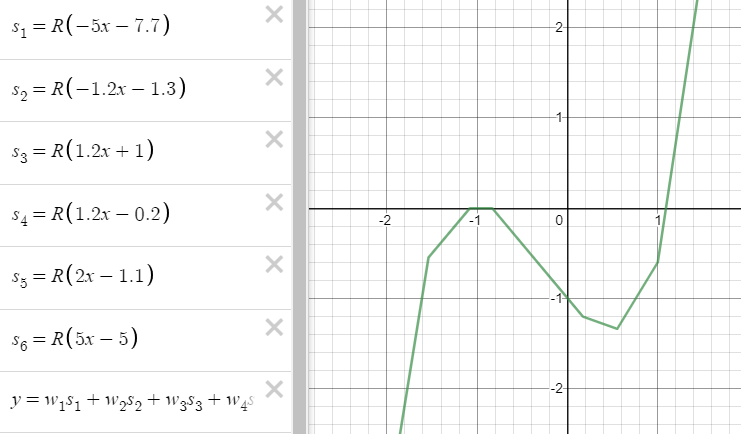
\includegraphics[height=5cm]{PPT/UniversalApproximationTheorem.png}
        \caption{A cubic function approximated by a neural network}\label{UniversalApproximationTheorem}
    The neural network used has 1 hidden layer containing 6 neurons.\\
    $R$ is an alias for the ReLU function (see Figure~\ref{ReLU}), and $y$ is the output layer neuron's activation value, obtained by summing over the product of the activation of the $i^{th}$ neuron $s_i$ with the weight of its connection to the final layer, $w_i$.
    \end{figure}
    Figure~\ref{fig:} Is a crude representation of how a 1-hidden-layer neural network can approximate a cubic function. A single hidden layer neural network with one scalar input and one scalar output is able to approximate any non-linear functions, provided that there are enough input and output neurons.
    (Explain adjusting bias leads to offset, and weights changes the slope, etc...)
    (Talk more about how this is a scalar func, not a vector field, etc. And interpolation is good, extrapolation is bad.)
    \subsubsection{Universal approximation theory}
    \begin{enumerate}
        \item general theory of neural network, and it's problems:
        \begin{itemize}
            \item explain in detail what is the structure of a Feed forward neural network, (act func, bias, weights)
            \item explain the need for normalization of features
            \item explain what is underfitting
            \item explain what is overfitting (the problem with memorization) (i.e. too many free paramters, so it just sits in a local minima that is slightly off from where it should be.)
            \item explain why it's important to keep the number of parameters low in order to minimize the problem of getting stuck at plateaus and saddle points (because of the unlikihood of minima)
            \item and list the hyperparameters that are tweaked in practice in order to make it more efficient.
            \begin{enumerate}
                 \item number of layers: generally a more complex problem requires more layers, e.g. more is required for facial recognitiion and differentiation than for a hand-written text classification engine.
                 \item activation function used
                 \item dropout (reduce connectedness of the NN)
                 \item weight regularlization
                 \item reduce learning rate on plateau
                 \item early stopping
                 \item etc... (whatever else I can think of)
             \end{enumerate}
        \end{itemize}
        \item this universal approximation theory can be applied in the M isotopes (M features) to N neutron groups (N labels), by making a k-layer neural networks, and list the hyperparameters that will/will not be tweaked:
        \begin{itemize}
            \item give an intuitive understanding of what's going on: mapping onto an N dimensional surface in a M dimensional volume/space?
            \item this works also because we expect it to find the (linear and non-linear components of) covariance between labels implicitly? Or is there more to it?
            \item in other words, it'll find where the bumps and dimples are on this ``surface", the orientation of this surface, etc. * (gotta think about this more)
            \item ASSUMING that we have a sufficient number of nuclear reactions to account for each of these components, and that the features (reaction rates) are noiseless, then a NN will be able to perfectly replicate it. 
            \item otherwise, a neural network may only be able to partially replicate these spectra, with poor quality
        \end{itemize}
    \end{enumerate}
    \subsubsection{The way that neural network will be applied in here:}
    What are labels, what are features.

    By assuming that invert to equation \ref{unfolding general equation} exist, i.e.

    \begin{equation} \label{unfolding inverse equation}
        \ve{Z} = \mathbf{\underline{\underline{R}}^{-1}} \ve{\phi_0}
    \end{equation}
    
    where the possible set of solution $\ve{Z}$ exist in an M-dimensional manifold in the N-dimensional space,

    \begin{itemize}
        \item approximate number of nodes per layer
        \item activation function to be used
        \item number of epochs to be used: 10000 or less, as it was observed
        \item number of layers:
        \item loss
    \end{itemize}
    \begin{itemize}
        \item neural network can work WITH or WITHOUT relying on the physics...
        \item here's it without relying on the physics...
        \item here's it with relying on the physics...
        Usually NN has fewer labels than features. Therefore the function to turn labels back into features doesn't always exist.

        But in this case, there are more labels than features. Therefore the function (denoted as $f$ as follows) that maps labels to feature exist (but not the other way around).
        
        Therefore, when using features to predict labels, we can generate, while trainig, the ``would-have-been" features from the predicted labels using $\text{feature}=f(\text{predicted labels})$, giving us yet another metric to train the neural network on, from which we expect to yield an increased learning rate as a result.
    \end{itemize}
    
    Plus the list of hyperparameters that will be kept constant/tweaked:
    \begin{itemize}
        \item num epochs: we do EarlyStopping instead
        \item num nodes:
        \item activation: always ReLU, since it's the standard, and to keep the number of tweaked hyperparamters simple
        \item loss function: pairwise, tried using cosine distance but it didn't work because it simply gave NaN's.
    \end{itemize}

\section{Literature review}
Previous attempts of machine learning techniques applied to unfolding only include:
\begin{itemize}
    \item Bonner spheres
    \item square matrices
    \item genetic algorithms
\end{itemize}
Therefore the neural network approach to unfolding the few-channel case is entirely new.

\section{Initial attempt on parameterised code}
For the simple 5$\times$5 case, did perfectly well.

But once we take log of both sides, it's become an impossible problem because we can't take log of a matrix that's singular. See Figure~\ref{5x5}.

\begin{figure}
\centering
\includegraphics[height=3cm]{/home/ocean/Documents/PTNR/CulhamFusion/Presentation2/FewChannels_fullydetermined/13simple_log.png}
\includegraphics[height=3cm]{/home/ocean/Documents/PTNR/CulhamFusion/Presentation2/FewChannels_fullydetermined/14simple_log.png}\\
\includegraphics[height=3cm]{/home/ocean/Documents/PTNR/CulhamFusion/Presentation2/FewChannels_fullydetermined/15simple_log.png}
\includegraphics[height=3cm]{/home/ocean/Documents/PTNR/CulhamFusion/Presentation2/FewChannels_fullydetermined/16simple_log.png}
\caption{The spectra predicted by a 2-hidden-layers neural network (with 16 nodes per layer) on a fully determined system.} \label{5x5}
% See /home/ocean/Documents/GitHubDir/unfolding/unfolding/unfoldingsuite/neuralnetwork/simplecase/log_simple_2_layer_error_variation.png for training progress graph
\end{figure}

% list of all spectra plotted together /home/ocean/Documents/GitHubDir/unfolding/AllSpec.png
\subsection{Creating simulated spectra by data augmentation}
To demonstrate that the neural network is capable of doing the unfolding procedure in an underdetermined condition, 1800 spectra were made to train the neural network.
%To create a large enough dataset, [explain parametrisation]
%Commonly used practice in Neural network is to introduce noise into the photos; But we can't just add random noise into the spectra and expect it to unfold the noise as well because adding meaningless information in case of an under-determined information condition will sqeeze away useful information out of the way.
Further increase in complexities (number of layers and numebr of nodes per layers) yield no significant improvement in the fit. This is because increasing the complexity further will simply lead to over-fitting, as the neural network `memorizes' the relationship between features and labels. This was reflected by the continual decrease in the loss value over the training data-set, while the loss value over the validation data-set stops improving.

\begin{figure}
\centering
    \begin{subfigure}[b]{.3\linewidth}
        \includegraphics[height=4cm]{/home/ocean/Documents/GitHubDir/unfolding/unfolding/unfoldingsuite/neuralnetwork/demogenerator/6_JET_FW_parametrised_spectrum_approximation_.png}
        \caption{An example of parametrisation performed on the JET spectra. These flux values are the total flux inside each energy bin, \emph{not} divided by the lethargy span of each bin, so they are higher/lower in wider/narrower energy bins.}
    \end{subfigure}
    \hfill
    \begin{subfigure}[b]{.65\linewidth}
        \includegraphics[height=7cm]{/home/ocean/Documents/GitHubDir/unfolding/unfolding/unfoldingsuite/neuralnetwork/_256_256_mse_training_spectra.png}
        \caption{300 $\times$ perturbed spectra were generated for each of the 6 original fusion spectra and plotted here, in flux per unit lethargy.}
    \end{subfigure}
\caption{Data augmentation performed to create simulated spectra.}\label{Parametrisation}
\end{figure}

\begin{figure}
\centering
    \begin{subfigure}[b]{11cm}
    \includegraphics[width=11cm]{/home/ocean/Documents/GitHubDir/unfolding/unfolding/unfoldingsuite/neuralnetwork/simulated_data/lossabove1e1/0918_0207_2_layer_256_256_mse_test_222_fluence.png}
    \caption{The neural network's predicted fluence was not normalized unlike the other two, therefore it was scaled up by a constant factor relative to the true fluence.}\label{SimulatedFluence}
    \end{subfigure}
    \begin{subfigure}[b]{5cm}
    \includegraphics[width=5cm]{/home/ocean/Documents/GitHubDir/unfolding/unfolding/unfoldingsuite/neuralnetwork/simulated_data/lossabove1e1/0918_0207_2_layer_256_256_mse_test_222_activities.png}
    \caption{The activities (features) used. The neural network was given the true activities, and asked to predict the fluence (\ref{SimulatedFluence}).
    \\Note that the colour scheme was reversed, i.e. the blue bars denote the activities predicted by the neural network instead of the true activities, and vice versa.
    }
    \end{subfigure}
\caption{The neural network's attempt at predicting a perturbed JET first wall spectrum.} \label{SimulatedExample}
\end{figure}
After being trained on variants of the same spectrum (only with slighly different peak heights), along with the perturbed spectra of 6 other fusion neutron sources.

It should be trying to approximate the underlying pattern,
In deed it does quite well.
But it's still not perfect.
Though that doesn't matter too much for our purpose. We deem it as good enough; move on.

\section{Attempt to work on the real data}

IF there's an underlying pattern, it will pick it out.
It performs just as well.

\subsection{Data attained}
Acquired from the IAEA UKAEA compendium.


Rebinning

\begin{figure}
\centering
\includegraphics[height=5cm]{/home/ocean/Documents/GitHubDir/unfolding/unfolding/unfoldingsuite/neuralnetwork/realoutputEarlyStopping/SelectedNNreplicated/real_fusion_train_spectra.png}
\caption{All fusion spectra used, obtained from \cite{ukaea_unfolding_support_report_march2017}}\label{RealFusionTrain}
\end{figure}

The neural networks were trained on 19 fusion neutron spectra, which were all rebinned into the Vitamin-J group structure.
How did you sort it

\begin{figure}
\centering
% \includegraphics[height=7cm]{/home/ocean/Documents/GitHubDir/unfolding/unfolding/referencesuite/175_group_test_set/ACT_raw_data/ACT_LogLogCrossSections.png}
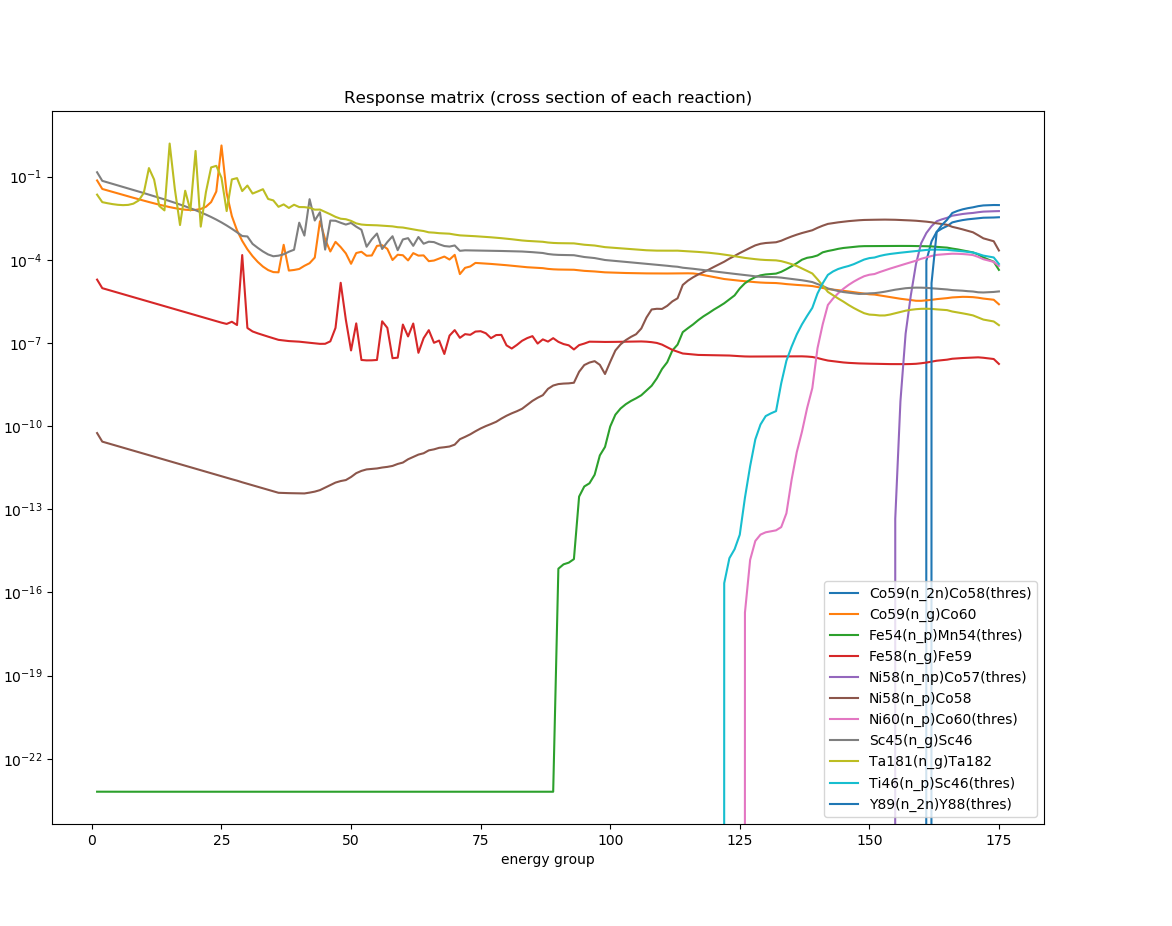
\includegraphics[height=7cm]{PPT/response_matrix.png}
\caption{Microscopic cross-section of each reaction}\label{response_matrix}
These values are obtained from TENDL15 via FISPACT-II \cite{FISPACT} at the left edge of each bin in the Vitamin-J group structure. 
\end{figure}
By assuming that the flux per unit lethargy inside each bin are relatively flat (energy independent), the activities contributed by the neutron flux in each bin is then proportional to the product of neutron flux with the microscopic. Symbolically,
\begin{equation} \label{unfolding proportional equation}
    Z_j \propto \sum_i \sigma_{ij} \phi_i
\end{equation}
Akin to the equation \ref{unfolding equation jth component}. Therefore these microscopic cross-section values were used in place of the response function for each of the reaction, assuming the constant of proportionality in equation \ref{unfolding proportional equation} is unity.
% No correction factors were applied as this is only a proof-of-concept experiment; applying correction factors that account for the number densities and foil volumes will only multiply the reaction rates by a fixed constant, thus effectively nullifying its effect.

\begin{figure}
\centering
\includegraphics[width=15cm]{/home/ocean/Documents/GitHubDir/unfolding/unfolding/unfoldingsuite/neuralnetwork/realoutputEarlyStopping/SelectedNNreplicated/fusion-fusion/mse_including_folded/fusion-fusion_mse_inc_folded_test_loss.png}
\caption{By visualizing the loss values attained by each neural network using a heatmap, the neural network which perform the best can be identified. For this particular heatmap, the loss value of the neural network's prediction on the test dataset (a set of fusion spectra that it has never seen before) is visualized, with darker colours representing lower loss values (good performance), vice versa. At the top right hand corner, i.e. the neural network with the hyperparameters of (learning rate=0.01, number of nodes in each layer=[32,53,90,152,256]), a particularly loss value is obtained. Therefore this neural network is regarded as the neural network with the optimal hyperparameter, and further investigation into the predictions of this neural network is conducted to see if it is purely coincidental or not.
}\label{hyperparametersearchTestLoss}
\end{figure}

\begin{figure}
\centering
\fluenceandactivities{/home/ocean/Documents/GitHubDir/unfolding/unfolding/unfoldingsuite/neuralnetwork/realoutputEarlyStopping/SelectedNNreplicated/fusion-fusion/0918_0332_5_layer_top_right_anomaly_test_001_}
\caption{}\label{5Layerfusion-fusionJET-FW}
\end{figure}

\begin{figure}
\centering
\fluenceandactivities{/home/ocean/Documents/GitHubDir/unfolding/unfolding/unfoldingsuite/neuralnetwork/realoutputEarlyStopping/SelectedNNreplicated/fusion-fusion/0918_0332_3_layer_typical_mpse_test_001_}
\caption{While other neural networks struggles to keep a close match to the profile. This neural network is Even though the neural netwrok attempts to follow the general rise-and-fall of the true spectrum, it does not follow the true spectrum's gradient closely enough, leading to extreme discrepancies at some bins (e.g. above 14.1MeV).}\label{3Layerfusion-fusionJET-FW}
\end{figure}

This shows that Figure~\ref{5Layerfusion-fusionJET-FW} likely only achieves the above average performance serendipiteously by re-tracing the same average spectrum. This hypothesis is supported by it replicating a very similar spectrum when it attempts to deduce the spectra corresponding to the other two test data.

% \begin{figure}
% \centering
% \fluenceandactivities{/home/ocean/Documents/GitHubDir/unfolding/unfolding/unfoldingsuite/neuralnetwork/realoutputEarlyStopping/SelectedNNreplicated/fusion-fusion/0918_0332_5_layer_top_right_anomaly_test_001_}
% \caption{}\label{5Layerfusion-fusionWCCB-FW}
% \end{figure}

% \begin{figure}
% \centering
% \fluenceandactivities{/home/ocean/Documents/GitHubDir/unfolding/unfolding/unfoldingsuite/neuralnetwork/realoutputEarlyStopping/SelectedNNreplicated/fusion-fusion/0918_0332_5_layer_top_right_anomaly_test_001_}
% \caption{}\label{5Layerfusion-fusionHCLL-VV}
% \end{figure}

% \begin{figure}
% \centering
% \fluenceandactivities{/home/ocean/Documents/GitHubDir/unfolding/unfolding/unfoldingsuite/neuralnetwork/realoutputEarlyStopping/SelectedNNreplicated/fusion-fusion/0918_0332_5_layer_top_right_anomaly_test_000_}
% \caption{}\label{5Layerfusion-fusionFNG}
% \end{figure}

% Regardless, we think it might be useful to make it a 

- What work has been done to find the optimal

- How to quantify optimal

\subsection{potential future improvements}
1. In the future we can calculate the spectral index, and plug THOSE values in, instead of plugging in the direct values, it might be better at picking out these differences, because it may be more obvious, and can pick it out even under so few data.

\section{Benchmarking against existing codes}
\subsection{As an unfolding tool}
If they would like to use it directly as an unfolding tool, then they can incorperate the whole folding process into the loss function; but this method requires:
\begin{itemize}
    \item (optional) The response matrix to already been known $\rightarrow$ better results?
\end{itemize}
*Gotta make a fair comparison between a neural network unfolded against an a priori unfolded one.

The more exciting aspect arises from the fact that it can be used as an a priori generator code:
\subsection{As an a priori generator}
Can be used as the a priori generator when:
\begin{figure}
\centering
\fluenceandactivities{/home/ocean/Documents/GitHubDir/unfolding/unfolding/unfoldingsuite/neuralnetwork/realinputEarlyStopping/comparison/real_fusion_test_gravel_nn_a_priori_test_001_}
\caption{But it also sucks as an a priori generator, giving a loss value of 9.89936, which is only a marginal improvement on the 10.188233 stated in Figure~\ref{gravel_flat_a_priori_JET}}\label{gravel_nn_a_priori_JET}
\end{figure}

\begin{figure}
\centering
\fluenceandactivities{/home/ocean/Documents/GitHubDir/unfolding/unfolding/unfoldingsuite/neuralnetwork/realinputEarlyStopping/comparison/real_fusion_test_gravel_test_001_}
\caption{Which is even worse than naive prior, i.e. using a flat a priori and thus giving no meaningful information to gravel before unfolding. In this case it achieves an average mean squared error of 10.188233}\label{gravel_flat_a_priori_JET}
\end{figure}

\begin{itemize}
    \item the user doesn't want to commit to hours of MCNP model generation (cite a paper where Lee Packer's group has used a whole MCNP model to get the response matrix and the reaction rates);
    \item and already has a few similar neutron spectra to pick from;
    \item want a higher reproducibility/credibility than hand-drawing an a priori with reference to the previous spectra/ averaging over the existing spectra.
\end{itemize}

EVEN if the response matrix is not known.

Allows for a probability distribution of weights? does that account for the variance and covariance between the labels and features? *
But this is beyond the scope of this paper, which is to demonstrate that the idea of NN works.

\section{An attempt at using fission data to predict fusion data}
Explain why: we have so many fission spectra... but only very few fusion spectra

But even the best neural network trained on fission spectra and obtained the lowest loss value when tested on fusion spectra gave very poor results:
\begin{figure}
\centering
\fluenceandactivities{/home/ocean/Documents/GitHubDir/unfolding/unfolding/unfoldingsuite/neuralnetwork/realoutputEarlyStopping/SelectedNNreplicated/fission-fusion/0918_0325_5_layer_test_mse_1_test_016_}
\caption{loss value still average to 43.33816909790039} \label{fission-fusionBad}
\end{figure}

\begin{figure}
\centering
\fluenceandactivities{/home/ocean/Documents/GitHubDir/unfolding/unfolding/unfoldingsuite/neuralnetwork/realoutputEarlyStopping/SelectedNNreplicated/fission-fusion/0918_0325_5_layer_test_mse_1_test_006_}
\caption{the best one looks like this}\label{fission-fusionGood}
\end{figure}

For the record, this optimal neural network has the hyperparameters of (learning rate = 0.01, number of nodes in each layer=[32,53,90,152,256]).

\section{Future improvements}
\begin{itemize}
    \item Transfer learning: start with fission data, fix the weights of the second half of the matrix as it gives the connection
    \item Use RBF NN or GRNN, which are known to perform better under low sample number conditions, though it is more complicated to implement.
    \item infer the uncertainty ($\sigma$) associated with the neural network's prediction using Monte Carlo method
\end{itemize}

\section{Conclusion}
\begin{itemize}
    \item What's the loss values
    \item achieved using what structure of NN
    \item trained upon what data
    \item How does it compare to neutron spectrum unfolding using other methods
    \item What's the significance on the unfolding community: should they use it more? Should they improve upon it?
    \item what additional observation did you find regarding training on different dataset.
\end{itemize}

\bibliographystyle{plain}
\bibliography{FACTIUNN}

\begin{appendices}

\section{Neural network building functions tailored for the purpose of neutron spectrum unfolding}
The following contains the class in which the neural network is built.\\
\pythoncode{neuralnetworklibrary.py}{/home/ocean/Documents/GitHubDir/unfolding/unfolding/unfoldingsuite/neuralnetwork/neuralnetworklibrary.py}

\section{Neural network abstractions and controller}
The following contains the higher level abstractions, as well as functions which walks the user through the process of creating a neural network interactively.\\
\pythoncode{neuralnetworktrainer.py}{/home/ocean/Documents/GitHubDir/unfolding/unfolding/unfoldingsuite/neuralnetwork/neuralnetworktrainer.py}

\section{Code for benchmarking}
This code uses 'unfoldingsuite', which contains implementations of MAXED and GRAVEL in python, developed locally at CCFE, to unfold spectra from various a priori. Their performance can then be used as benchmarks for the neural network unfolding results to be compared against.\\
\pythoncode{comparison\_with\_existing.py}{/home/ocean/Documents/GitHubDir/unfolding/unfolding/unfoldingsuite/neuralnetwork/realinputEarlyStopping/comparison/comparison_with_existing.py}

\section{Fully determined simulation data generation}
Creates a 5 energy-bins fluence vector, which is then folded through a 5 $\times$ 5 response matrix; both of which are randomly generated. Each element both were picked from a uniform random distribution larger than 1. The upper bound of the elements in the vector were chosen as 15 and the upper bound of the elements in the response matrix were chosen to be 50.\\
\pythoncode{simple\_non\_singular\_case.py}{/home/ocean/Documents/GitHubDir/unfolding/unfolding/unfoldingsuite/neuralnetwork/demogenerator/simple_non_singular_case.py}

\section{Underdetermined simulation data generation}
For each of the 14 FISPACT reference spectra, each is parametrised into a list of peaks. The height of these peaks were then perturbed to form a `new' spectrum. This `new' spectrum is then folded through a corresponding response matrix.\\
\pythoncode{spectrumrandomizer.py}{/home/ocean/Documents/GitHubDir/unfolding/unfolding/unfoldingsuite/neuralnetwork/demogenerator/spectrumrandomizer.py}

\section{Training and evaluating neural networks on the underdetermined simulation data}
A demonstration of applying neuralnetworktrainer.py on the data generated by spectrumrandomizer.py .\\
\pythoncode{script\_for\_demo.py}{/home/ocean/Documents/GitHubDir/unfolding/unfolding/unfoldingsuite/neuralnetwork/script_for_demo.py}

%IAEA and UKAEA compendium spectra had to be rebinned into the vitamin J spectra in order to be useful.

\section{Selecting from UKAEA and IAEA compendium}
Rebinned spectra from the 212 IAEA + UKAEA compendium were sorted into various training and testing sets using the following python program.\\
\pythoncode{getrealdata.py}{/home/ocean/Documents/GitHubDir/unfolding/unfolding/unfoldingsuite/neuralnetwork/Link_UKAEA_IAEA_Compendium/getrealdata.py}

\section{hyperparameter input controller}
Input files for hyperparametertrainer.py using the following code, by iterating through a list of hyperparameters of interest, thus effectively performing a grid search over all hyperparameters.\\
\pythoncode{hyperparameterinput.py}{/home/ocean/Documents/GitHubDir/unfolding/unfolding/unfoldingsuite/neuralnetwork/realinputEarlyStopping/hyperparameterinput.py}
This program can be used to split the into multiple jobs, which can then be submitted to a cluster, parallellizing the process and massively reducing the training and evaluation time of the neural networks. This is done by calling the program with \texttt{python hyperparameterinput.py split}

\section{hyperparameter optimization searching}
List the hyperparameter, training- and testing-sets used to evaluate the neural network on, when the hash\_name of the neural network is given.\\
\pythoncode{hyperparameteroutput.py}{/home/ocean/Documents/GitHubDir/unfolding/unfolding/unfoldingsuite/neuralnetwork/realoutputEarlyStopping/hyperparameteroutput.py}

\section{Loss value visualizer}
When given the names of the training- and testing-set, the following code show the loss values (and other metrics) of the neural networks with different hyperparameters achieved on them. This is plotted as a heat map, over the two dimensions of hyperparameters varied, which are `number of layers' (y-axis) and `learning rate' (x-axis) respectively.\\
\pythoncode{hyperparameteroptimizer.py}{/home/ocean/Documents/GitHubDir/unfolding/unfolding/unfoldingsuite/neuralnetwork/realoutputEarlyStopping/hyperparameteroptimizer.py}

\end{appendices}

\end{document}

% With data augmentation: it works quite well, even when there are only 2 layers.
%WIthout data augmentation: Suffer from a big problem of insufficient data.
%`